\documentclass[11pt,a4paper]{article}
\usepackage[utf8]{inputenc}
\usepackage[T1]{fontenc}
\usepackage[norsk]{babel}
\usepackage{tgtermes}
\usepackage{tgheros}
\renewcommand{\ttdefault}{txtt}
\usepackage{amsmath,amssymb}
\usepackage[a4paper,left=2.45cm,right=2.6cm,top=2.3cm,bottom=2.2cm,headsep=0.9cm]{geometry}
\usepackage{fancyhdr}
\usepackage{lastpage}
\usepackage{xcolor}
\usepackage{tikz}
\usepackage{pgfplots}
\pgfplotsset{compat=1.18}
\usepackage{booktabs}
\usepackage{array}
\usepackage{enumitem}
\usepackage{listings}
\usepackage{needspace}
\usepackage{multirow}
\usetikzlibrary{positioning,arrows.meta,calc}
\definecolor{insgrey}{gray}{0.42}
\definecolor{radiogrey}{gray}{0.70}
\setlength{\parindent}{0pt}
\setlength{\parskip}{0.45em}
\setlist[itemize]{itemsep=0pt,topsep=2pt,label=\textbullet,font=\sffamily}
\lstset{basicstyle=\ttfamily\small,columns=fullflexible,keepspaces=true,
  showstringspaces=false,upquote=true,aboveskip=0.6em,belowskip=0.6em,
  literate={æ}{{\ae}}1 {ø}{{\o}}1 {å}{{\aa}}1 {Æ}{{\AE}}1 {Ø}{{\O}}1 {Å}{{\AA}}1}
\pagestyle{fancy}
\fancyhf{}
\renewcommand{\headrulewidth}{0pt}
\fancyhead[R]{\fontsize{7.5}{9}\selectfont\sffamily\color{insgrey}TDT4172 - Introduksjon til maskinlæring - Øvingssett 3}
\fancyfoot[R]{\fontsize{7}{9}\selectfont\sffamily\color{insgrey}\thepage/\pageref{LastPage}}
\newcommand{\delstart}[1]{\clearpage
  \noindent\hspace*{-1.55em}\makebox[1.55em][l]{\sffamily\bfseries\fontsize{12}{14}\selectfont\raisebox{0.35em}{#1}}%
  {\sffamily\bfseries\fontsize{18}{22}\selectfont Part #1}\par\vspace{1.0em}}
\newcommand{\sporsmal}[1]{\par\Needspace{9\baselineskip}\vspace{1.9em}%
  \noindent{\bfseries Spørsmål #1}\par\vspace{-0.45em}%
  \noindent{\bfseries -{}-{}-{}-{}-{}-{}-{}-{}-{}-{}-{}-{}-{}-{}-{}-{}-}\par\vspace{-0.15em}}
\newcommand{\velg}[1]{\par\Needspace{6\baselineskip}\noindent{\bfseries #1}\par\vspace{0.3em}}
\newcommand{\radio}[1]{\tikz[baseline=-0.62ex]{\draw[radiogrey,line width=0.45pt,fill=gray!5] (0,0) circle (0.56em);
  \node[inner sep=0pt,font=\sffamily\fontsize{5.5}{6}\selectfont,text=insgrey] at (0,0) {#1};}}
\newenvironment{alternativer}{\begin{list}{}{\setlength{\leftmargin}{2.35em}\setlength{\labelwidth}{1.4em}%
  \setlength{\labelsep}{0.6em}\setlength{\itemsep}{0.85em}\setlength{\topsep}{0.45em}\setlength{\parsep}{0pt}}%
  \sffamily\fontsize{10}{12.6}\selectfont}{\end{list}}
\newcommand{\alt}[2]{\item[\radio{#1}]#2}
\newcommand{\makspoeng}{\par\vspace{2.2em}\hfill{\sffamily\fontsize{8.5}{10}\selectfont Maks poeng: 10}\hspace*{0.5em}\par}
\begin{document}

\noindent\hspace*{-1.55em}\makebox[1.55em][l]{\raisebox{0.3em}{\sffamily\bfseries\fontsize{11}{12}\selectfont i}}%
{\sffamily\bfseries\fontsize{18}{22}\selectfont Frontpage}\par\vspace{1.1em}

{\bfseries Eksamensoppgave i TDT4172 - Introduksjon til maskinlæring}\\
{\bfseries Øvingssett:} 3 av 10 (uoffisielt øvingssett)\\
{\bfseries Tid:} 4 timer

\vspace{0.6em}
{\bfseries Faglig kontakt:} --- (øvingssett, ikke en offisiell eksamen)\\
{\bfseries Møter i eksamenslokalet:} Nei

\vspace{0.6em}
{\bfseries Hjelpemiddelkode/Tillatte hjelpemidler:} D / Ingen trykte eller håndskrevne hjelpemidler tillatt.
Bestemt, enkel kalkulator tillatt.

\vspace{0.6em}
{\bfseries\underline{ANNEN INFORMASJON:}}

\vspace{0.4em}
{\bfseries Les oppgavene nøye og gjør dine egne antagelser.} Presiser i besvarelsen hvilke forutsetninger du
har lagt til grunn i tolkning/avgrensing av oppgaven.

Dette øvingssettet er laget for egentrening, med samme format og vanskelighetsgrad som de
siste ordinære eksamenene i emnet. Løsningsforslaget står på siste side.

\vspace{1.6em}
{\bfseries\underline{FAGSPESIFIKK INFORMASJON}}

\vspace{0.4em}
{\bfseries Ingen papirhåndtegninger:}\\
Denne eksamenen tillater ikke bruk av håndtegninger.

\vspace{1.4em}
{\bfseries Vekting av oppgavene}:\\
Denne eksamenen inneholder flervalgsoppgaver organisert i ti grupper på fire spørsmål hver. Hver
gruppe vurderes separat etter følgende regler:

\vspace{0.6em}
For hver av de fire spørsmålene i gruppen får du følgende poeng
\begin{itemize}[leftmargin=2.2em,label=\textperiodcentered,itemsep=0pt]
\item {\bfseries Riktig svar:} +2,5 poeng
\item {\bfseries Feil svar (et alternativ er valgt, men ikke korrekt):} $-$0,83 poeng
\item {\bfseries Ikke besvart:} 0 poeng
\end{itemize}
{\bfseries Merk} at dersom du først har valgt et svaralternativ, kan du {\bfseries ikke velge det bort} igjen. Da må du
svare på det spørsmålet. Med andre ord mister du muligheten til å la et spørsmål stå blankt så fort
du har trykket på et alternativ.

\vspace{0.6em}
Poengsummen for hver gruppe er {\bfseries summen} av poengene for de fire enkeltspørsmålene.\\
For {\bfseries alle spørsmålene} gjelder en {\bfseries null-grense}: dersom summen for denne gruppen blir negativ,
settes verdien til {\bfseries 0}. Den totale poengsummen på eksamen er summen av poengene fra alle
gruppene.

\delstart{1}
\sporsmal{1}
En \textbf{logistisk regresjonsmodell} med to features predikerer
\[ \hat y = \sigma(w_1 x_1 + w_2 x_2 + b), \]
og klassifiserer et punkt som positivt når $\hat y > 0.5$.

Hvilket utsagn om \textbf{beslutningsgrensen} til denne modellen er korrekt?
\velg{Velg ett alternativ:}
\begin{alternativer}
\alt{A}{Den er linjen $w_1x_1 + w_2x_2 + b = 0.5$, fordi terskelen for klassifisering er 0.5}
\alt{B}{Den er S-formet i $(x_1, x_2)$-planet, fordi sigmoid-funksjonen er ikke-lineær}
\alt{C}{Den er linjen $w_1x_1 + w_2x_2 + b = 0$, fordi $\sigma(z) = 0.5$ nøyaktig når $z = 0$}
\alt{D}{Den kan bli krum dersom modellen trenes lenge nok med gradient descent}
\end{alternativer}
\sporsmal{2}
En modell gir prediksjonene under for to datapunkter. Tapet er gjennomsnittlig
\textbf{binary cross-entropy} med naturlig logaritme,
$L = -\frac{1}{N}\sum_i \big[\,y_i \ln \hat y_i + (1-y_i)\ln(1-\hat y_i)\,\big]$.
Punkt 1 har $y = 1$ og $\hat y = 0.8$, og punkt 2 har $y = 0$ og $\hat y = 0.6$.

Hva blir tapet $L$?
\velg{Velg ett alternativ:}
\begin{alternativer}
\alt{A}{$0.37$}
\alt{B}{$0.25$}
\alt{C}{$0.11$}
\alt{D}{$0.57$}
\end{alternativer}
\sporsmal{3}
I logistisk regresjon er $\hat y = \sigma(z)$ med $z = \mathbf{w}^T\mathbf{x} + b$. For et bestemt datapunkt
gir modellen $\hat y = 0.8$.

Hva er verdien av $z$ for dette punktet?
\velg{Velg ett alternativ:}
\begin{alternativer}
\alt{A}{$z \approx -0.22$}
\alt{B}{$z \approx 1.39$}
\alt{C}{$z \approx 0.69$}
\alt{D}{$z \approx 0.60$}
\end{alternativer}
\sporsmal{4}
En logistisk regresjonsmodell med tre features, $\hat y = \sigma(w_1x_1 + w_2x_2 + w_3x_3 + b)$, trenes med
gradient descent på 500 treningspunkter.

I hvilket rom tar gradient descent stegene sine, og hvor mange dimensjoner har det?
\velg{Velg ett alternativ:}
\begin{alternativer}
\alt{A}{I rommet av treningspunkter, med én dimensjon per punkt, altså 500 dimensjoner}
\alt{B}{I feature-rommet spent ut av $(x_1, x_2, x_3)$, som har tre dimensjoner}
\alt{C}{I prediksjonsrommet til $\hat y$, som har én dimensjon siden $\hat y \in (0,1)$}
\alt{D}{I parameterrommet spent ut av $(w_1, w_2, w_3, b)$, som har fire dimensjoner}
\end{alternativer}
\makspoeng

\delstart{2}
\sporsmal{1}
En binær klassifikator gir en score $\hat y \in (0,1)$, og et punkt klassifiseres som positivt når
$\hat y > t$. \textbf{ROC-kurven} lages ved å variere terskelen $t$ fra 1 til 0.

Hvilket utsagn om ROC-kurven er korrekt?
\velg{Velg ett alternativ:}
\begin{alternativer}
\alt{A}{En modell som gjetter tilfeldig gir kurven $\mathrm{TPR} = 1 - \mathrm{FPR}$}
\alt{B}{Med $t = 0$ havner modellen alltid i punktet $(\mathrm{FPR}, \mathrm{TPR}) = (1, 1)$}
\alt{C}{Et punkt over diagonalen betyr at modellen har flere falske positive enn sanne positive}
\alt{D}{Med $t = 1$ havner modellen i punktet $(\mathrm{FPR}, \mathrm{TPR}) = (0, 1)$}
\end{alternativer}
\sporsmal{2}
En klassifikator gir skår $s \in (0,1)$, og et punkt klassifiseres som positivt når skåren er over 0.5.
Uten å trene noe på nytt erstatter en kollega alle skårene med $s^2$ før evalueringen på testsettet.
Terskelen holdes på 0.5.

Hva skjer med metrikkene sammenlignet med de opprinnelige skårene?
\velg{Velg ett alternativ:}
\begin{alternativer}
\alt{A}{ROC AUC og accuracy ved terskel 0.5 kan begge endres, siden skårene har fått nye verdier}
\alt{B}{ROC AUC og accuracy ved terskel 0.5 er begge uendret, siden modellen ikke er trent på nytt}
\alt{C}{ROC AUC synker fordi alle skårene blir lavere, mens accuracy ved terskel 0.5 er uendret}
\alt{D}{ROC AUC er uendret fordi rekkefølgen av skårene bevares, mens accuracy ved terskel 0.5 kan endres}
\end{alternativer}
\sporsmal{3}
Tabellen viser score og sann klasse for ti testpunkter. Et punkt klassifiseres som positivt når
score $> 0.6$.

\begin{center}
\begin{tabular}{l*{10}{c}}
\toprule
Score & 0.95 & 0.85 & 0.80 & 0.70 & 0.65 & 0.55 & 0.45 & 0.40 & 0.30 & 0.10 \\
Sann klasse & 1 & 0 & 1 & 1 & 0 & 0 & 1 & 0 & 0 & 0 \\
\bottomrule
\end{tabular}
\end{center}

Hvilket punkt $(\mathrm{FPR}, \mathrm{TPR})$ på ROC-kurven svarer denne terskelen til?
\velg{Velg ett alternativ:}
\begin{alternativer}
\alt{A}{$(0.40,\ 0.60)$}
\alt{B}{$(0.33,\ 0.75)$}
\alt{C}{$(0.67,\ 0.25)$}
\alt{D}{$(0.20,\ 0.30)$}
\end{alternativer}
\sporsmal{4}
For en binær klassifikator ved en gitt terskel er antall \textbf{true positives} $\mathrm{TP} > 0$.

Hvilken betingelse gjør at \textbf{precision} og \textbf{recall} blir like store?
\velg{Velg ett alternativ:}
\begin{alternativer}
\alt{A}{Antall falske positive er lik antall sanne negative}
\alt{B}{Antallet sanne positive er lik antallet sanne negative}
\alt{C}{Antall falske positive er lik antall falske negative}
\alt{D}{Antall sanne negative er lik antall falske negative}
\end{alternativer}
\makspoeng

\delstart{3}
\sporsmal{1}
Et Naive Bayes-filter for søppelpost estimerer $p(x_i \mid C_k)$ som relative frekvenser i treningsdataene.
Ordet «kryptogevinst» finnes i flere søppel-e-poster, men aldri i en vanlig e-post i treningsdataene.
En ny jobb-e-post inneholder dette ordet én gang; alle de andre ordene i den finnes i begge klassene.

Hva skjer når filteret klassifiserer den nye e-posten?
\velg{Velg ett alternativ:}
\begin{alternativer}
\alt{A}{Ordet ignoreres, siden det bare finnes i én av klassene og derfor ikke kan brukes til å skille dem}
\alt{B}{Prioren $p(\text{vanlig})$ settes til 0, men de andre ordene i e-posten kan likevel gi klassen «vanlig»}
\alt{C}{E-posten havner i klassen med høyest prior, siden én av likelihoodene er udefinert}
\alt{D}{Produktet for klassen «vanlig» blir 0, så e-posten blir alltid klassifisert som søppel}
\end{alternativer}
\sporsmal{2}
En løvnode i et klassifiseringstre med \textbf{tre klasser} inneholder 10 punkter: 5 fra klasse A, 3 fra
klasse B og 2 fra klasse C.

Hva er Gini-urenheten $1 - \sum_i p_i^2$ i noden?
\velg{Velg ett alternativ:}
\begin{alternativer}
\alt{A}{$0.50$}
\alt{B}{$0.42$}
\alt{C}{$0.38$}
\alt{D}{$0.62$}
\end{alternativer}
\sporsmal{3}
Figuren viser et beslutningstre som predikerer kjønnet til pingviner i Palmer Penguins-dataene fra
kroppsmasse $m$ (gram) og flipperlengde $f$ (mm). I hver beslutningsnode går punkter som oppfyller
betingelsen til venstre (ja), og de andre til høyre (nei).
\begin{center}
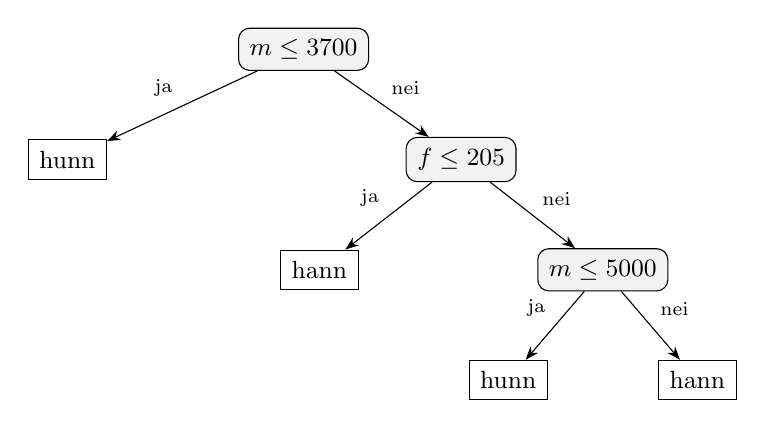
\begin{tikzpicture}[
  every node/.style={font=\small},
  beslut/.style={draw, rounded corners, fill=gray!10, inner sep=4pt},
  lov/.style={draw, inner sep=4pt},
  edge/.style={-{Stealth}}]
\node[beslut] (r) at (0,0) {$m \le 3700$};
\node[lov] (l1) at (-3,-1.4) {hunn};
\node[beslut] (n2) at (2,-1.4) {$f \le 205$};
\node[lov] (l2) at (0.2,-2.8) {hann};
\node[beslut] (n3) at (3.8,-2.8) {$m \le 5000$};
\node[lov] (l3) at (2.6,-4.2) {hunn};
\node[lov] (l4) at (5.0,-4.2) {hann};
\draw[edge] (r) -- node[above left, font=\scriptsize] {ja} (l1);
\draw[edge] (r) -- node[above right, font=\scriptsize] {nei} (n2);
\draw[edge] (n2) -- node[above left, font=\scriptsize] {ja} (l2);
\draw[edge] (n2) -- node[above right, font=\scriptsize] {nei} (n3);
\draw[edge] (n3) -- node[above left, font=\scriptsize] {ja} (l3);
\draw[edge] (n3) -- node[above right, font=\scriptsize] {nei} (l4);
\end{tikzpicture}
\end{center}
Hvilken beskrivelse gir nøyaktig de pingvinene som treet predikerer som hann?
\velg{Velg ett alternativ:}
\begin{alternativer}
\alt{A}{$m > 3700$ og $f \le 205$, eller $m > 5000$ og $f > 205$}
\alt{B}{$f \le 205$ uansett masse, eller $m > 5000$ og $f > 205$}
\alt{C}{$m > 3700$ og $f > 205$, eller $m > 5000$ og $f \le 205$}
\alt{D}{$m > 3700$ og $f \le 205$, eller $m \le 5000$ og $f > 205$}
\end{alternativer}
\sporsmal{4}
En node i et beslutningstre har 8 positive og 2 negative datapunkter. En kandidatsplitt gir venstre barn
med 2 positive og 2 negative, og høyre barn med 6 positive og 0 negative. Entropien er
$I = -\sum_i p_i \log_2 p_i$, og informasjonsgevinsten er $\Delta I = I_{\text{før}} - E[I_{\text{etter}}]$,
der $E[I_{\text{etter}}]$ vekter hvert barn med andelen av punktene.

Hvilket utsagn om denne splitten er riktig?
\velg{Velg ett alternativ:}
\begin{alternativer}
\alt{A}{Entropien etter splitten er 0.5, snittet av barnas entropi, og dermed lavere enn før splitten}
\alt{B}{Venstre barn har høyere entropi enn foreldrenoden, så informasjonsgevinsten blir negativ}
\alt{C}{Venstre barn har høyere entropi enn foreldrenoden, men informasjonsgevinsten er likevel positiv}
\alt{D}{Begge barna har lavere entropi enn foreldrenoden, slik det alltid blir etter en binær splitt}
\end{alternativer}
\makspoeng

\delstart{4}
\sporsmal{1}
Regresjonstrær med ulik maksimal dybde trenes på samme data. Tabellen viser MSE på trenings- og
valideringsdata.

\begin{center}
\begin{tabular}{lcc}
\toprule
Maks dybde & Trenings-MSE & Validerings-MSE \\
\midrule
1 & 41.0 & 43.0 \\
3 & 12.0 & 15.0 \\
8 & 4.0 & 13.0 \\
20 & 0.0 & 38.0 \\
\bottomrule
\end{tabular}
\end{center}

Hvilket utsagn er korrekt?
\velg{Velg ett alternativ:}
\begin{alternativer}
\alt{A}{Treet med dybde 1 undertilpasser, siden feilen er høy både på trening og validering}
\alt{B}{Treet med dybde 20 undertilpasser, siden treningsfeilen ikke kan bli lavere enn 0.0}
\alt{C}{Treet med dybde 20 er best, siden det har lært sammenhengen i treningsdataene perfekt}
\alt{D}{Treet med dybde 1 overtilpasser, siden trenings- og valideringsfeilen er nesten like store}
\end{alternativer}
\sporsmal{2}
Figuren viser trenings- og valideringstap for et nevralt nettverk over 100 epoker.

\begin{center}
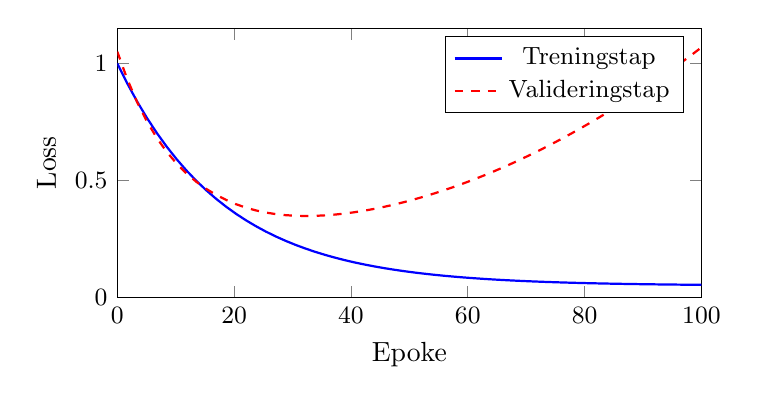
\begin{tikzpicture}
\begin{axis}[width=9cm,height=5cm,xlabel={Epoke},ylabel={Loss},xmin=0,xmax=100,ymin=0,ymax=1.15,
  legend style={font=\small,at={(0.97,0.97)},anchor=north east},tick label style={font=\small}]
\addplot[blue,thick,domain=0:100,samples=60] {0.05+0.95*exp(-x/18)};
\addlegendentry{Treningstap}
\addplot[red,thick,dashed,domain=0:100,samples=60] {0.30+0.75*exp(-x/10)+0.00012*max(0,x-20)^2};
\addlegendentry{Valideringstap}
\end{axis}
\end{tikzpicture}
\end{center}

Hva er den mest rimelige tolkningen og det beste tiltaket?
\velg{Velg ett alternativ:}
\begin{alternativer}
\alt{A}{Valideringssettet er for lite; slå det sammen med testsettet og velg epoke ut fra testtapet}
\alt{B}{Modellen overtilpasser fra ca.\ epoke 30; early stopping på valideringstapet stanser treningen der}
\alt{C}{Modellen undertilpasser, siden valideringstapet er høyere enn treningstapet; tren i flere epoker}
\alt{D}{Læringsraten er for høy, siden valideringstapet øker; senk læringsraten og tren i 100 epoker til}
\end{alternativer}
\sporsmal{3}
Data genereres som $y = F(x) + \varepsilon$, der $\varepsilon$ har forventning 0 og varians $\sigma^2 = 4$.
En modell evalueres med forventet kvadratfeil $E\big[(y - f(x;D))^2\big]$ på nye datapunkter.

Hvilket utsagn er korrekt?
\velg{Velg ett alternativ:}
\begin{alternativer}
\alt{A}{Forventet kvadratfeil kan bli 0 med en modell som har høy nok kompleksitet}
\alt{B}{Forventet kvadratfeil kan bli vilkårlig lav dersom vi samler inn nok treningsdata}
\alt{C}{Forventet kvadratfeil kan ikke bli lavere enn 2, som er standardavviket til støyen}
\alt{D}{Forventet kvadratfeil kan aldri bli lavere enn 4, uansett modell og datamengde}
\end{alternativer}
\sporsmal{4}
Du trener en lineær regresjonsmodell med \textbf{stochastic gradient descent} (ett datapunkt per
oppdatering) og konstant læringsrate $\eta = 0.05$. Treningstapet synker raskt de første epokene,
men blir deretter liggende og hoppe opp og ned rundt omtrent samme nivå. En kollega foreslår å la
$\eta$ avta gradvis i løpet av treningen.

Hva er den beste begrunnelsen for forslaget?
\velg{Velg ett alternativ:}
\begin{alternativer}
\alt{A}{Gradienten vokser når parametrene nærmer seg minimum, så læringsraten må ned for at tapet ikke skal begynne å divergere igjen}
\alt{B}{Svingningene skyldes overtilpasning, og en avtagende læringsrate virker som early stopping som hindrer tilpasning til støyen}
\alt{C}{Store steg gir rask fremgang tidlig i treningen, mens små steg senere lar parametrene slå seg til ro nær minimum}
\alt{D}{Mindre steg mot slutten gjør tapsflaten konveks, slik at gradient descent ikke kan bli sittende fast i et lokalt minimum}
\end{alternativer}
\makspoeng

\delstart{5}
\sporsmal{1}
Boosting-algoritmer som AdaBoost bruker ofte \textbf{trestumper} som enkeltmodeller.

Hvorfor fungerer dette godt?
\velg{Velg ett alternativ:}
\begin{alternativer}
\alt{A}{Hver stump har høy bias, og boosting reduserer bias ved å kombinere mange stumper sekvensielt}
\alt{B}{Stumpene trenes parallelt og uavhengig av hverandre, slik at ensemblet blir raskt å trene}
\alt{C}{Stumpene trenes på ulike bootstrap-utvalg, slik at de blir mindre korrelerte med hverandre}
\alt{D}{Hver stump har høy varians, og boosting reduserer varians ved å ta gjennomsnitt av uavhengige stumper}
\end{alternativer}
\sporsmal{2}
I første runde av \textbf{AdaBoost} har alle de 10 treningspunktene vekt $0.1$. Den første stumpen
klassifiserer punkt 3 og punkt 7 feil, og resten riktig.

Hva skjer før neste stump trenes?
\velg{Velg ett alternativ:}
\begin{alternativer}
\alt{A}{Alle punktene beholder vekt 0.1, men stumpens stemmevekt justeres etter feilraten}
\alt{B}{Punkt 3 og 7 får lavere vekt, siden feilklassifiserte punkter trolig er støy}
\alt{C}{Punkt 3 og 7 får høyere vekt, så neste stump legger mer vekt på å få dem riktig}
\alt{D}{Neste stump trenes på residualene fra første stump, med lik vekt på alle punktene}
\end{alternativer}
\sporsmal{3}
Du trener en \textbf{random forest} med ulikt antall trær på de samme dataene og måler feilraten på
valideringsdata:
\begin{center}
\begin{tabular}{lcccc}
\toprule
Antall trær & 10 & 100 & 1000 & 5000 \\
\midrule
Valideringsfeil & 0.240 & 0.205 & 0.201 & 0.201 \\
\bottomrule
\end{tabular}
\end{center}
En kollega er bekymret for at 5000 trær vil overtilpasse, slik som når gradient boosting får for mange runder.

Hvilket utsagn er riktig?
\velg{Velg ett alternativ:}
\begin{alternativer}
\alt{A}{Flere trær gjør bare snittet over trærne mer stabilt, så feilen flater ut i stedet for å øke; prisen er regnetid}
\alt{B}{Feilen flater ut fordi bootstrap-utvalgene etter hvert blir identiske, så de siste trærne er kopier av de første}
\alt{C}{Med svært mange trær kan skogen gradvis overtilpasse, så 5000 trær bør unngås selv om feilen ennå ikke har økt}
\alt{D}{Hvert nytt tre retter feilene til de forrige trærne, så etter mange trær begynner skogen å tilpasse seg støy}
\end{alternativer}
\sporsmal{4}
Tabellen viser om hver av tre klassifikatorer predikerer riktig (1) eller feil (0) på seks testpunkter i
en binær klassifiseringsoppgave. De tre kombineres med flertallsavstemning.
\begin{center}
\begin{tabular}{lcccccc}
\toprule
Punkt & 1 & 2 & 3 & 4 & 5 & 6 \\
\midrule
Modell 1 & 1 & 1 & 1 & 1 & 1 & 0 \\
Modell 2 & 1 & 1 & 1 & 1 & 0 & 0 \\
Modell 3 & 1 & 1 & 1 & 0 & 0 & 1 \\
\bottomrule
\end{tabular}
\end{center}
Hva blir accuracy for ensemblet på disse seks punktene?
\velg{Velg ett alternativ:}
\begin{alternativer}
\alt{A}{$1.00$}
\alt{B}{$0.50$}
\alt{C}{$0.83$}
\alt{D}{$0.67$}
\end{alternativer}
\makspoeng

\delstart{6}
\sporsmal{1}
Et fullt koblet nettverk har tre skjulte lag, men \textbf{ingen aktiveringsfunksjon} (identitet) i noen
av lagene.

Hvilke sammenhenger mellom input og output kan nettverket representere?
\velg{Velg ett alternativ:}
\begin{alternativer}
\alt{A}{Kun konstante funksjoner, siden alle gradientene blir null uten en aktiveringsfunksjon}
\alt{B}{Kun lineære (affine) sammenhenger, siden flere lineære lag etter hverandre er lineært}
\alt{C}{Ikke-lineære sammenhenger, så lenge nettverket har minst to skjulte lag med flere noder}
\alt{D}{Polynomiske sammenhenger, siden hvert lag multipliserer inn en ny potens av input}
\end{alternativer}
\sporsmal{2}
Et fullt koblet nettverk har 8 input-features, to skjulte lag med henholdsvis 16 og 8 noder, og et
output-lag med 3 noder. Alle lag etter input-laget har bias.

Hvor mange trenbare parametre har nettverket?
\velg{Velg ett alternativ:}
\begin{alternativer}
\alt{A}{$307$}
\alt{B}{$280$}
\alt{C}{$283$}
\alt{D}{$304$}
\end{alternativer}
\sporsmal{3}
Et nettverk med \textbf{sigmoid}-aktivering i det skjulte laget initialiseres med alle vekter og bias lik 0.

Hva skjer når nettverket trenes med gradient descent?
\velg{Velg ett alternativ:}
\begin{alternativer}
\alt{A}{Symmetrien brytes etter første steg, fordi hver skjult node får ulike input-verdier fra dataene}
\alt{B}{Nodene i det skjulte laget får like oppdateringer og forblir identiske, så laget virker som én node}
\alt{C}{Alle gradienter blir null i hele nettverket, så ingen av parametrene endres under treningen}
\alt{D}{Treningen konvergerer raskere, fordi alle noder starter i samme punkt og deler gradienten}
\end{alternativer}
\sporsmal{4}
Output-laget i et klassifiseringsnettverk har tre noder med \textbf{softmax}-aktivering. Før aktivering er
verdiene $z = (1.5,\ 0.5,\ -1.0)$.

Hva blir den predikerte sannsynligheten for \emph{klasse 2} (den med $z_2 = 0.5$)?
\velg{Velg ett alternativ:}
\begin{alternativer}
\alt{A}{$0.62$}
\alt{B}{$0.25$}
\alt{C}{$0.69$}
\alt{D}{$0.50$}
\end{alternativer}
\makspoeng

\delstart{7}
\sporsmal{1}
Du sammenligner to klyngeinndelinger av samme datasett. Inndeling A har \textbf{Calinski--Harabasz-score}
850, mens inndeling B har 120.

Hvilket utsagn er korrekt?
\velg{Velg ett alternativ:}
\begin{alternativer}
\alt{A}{A har mest spredte klynger, siden scoren er summen av kvadrerte avstander til sentroidene}
\alt{B}{Scoren ligger alltid i $[-1, 1]$, så verdiene tyder på en feil i beregningen}
\alt{C}{B er best, siden lav score betyr liten avstand mellom punktene innad i klyngene}
\alt{D}{A har klynger som er bedre separert relativt til spredningen innad i klyngene}
\end{alternativer}
\sporsmal{2}
k-means med $k = 3$ brukes på de endimensjonale punktene $0,\ 2,\ 10,\ 12,\ 20,\ 22$.
Startsentroidene er $0$, $2$ og $16$, og algoritmen kjøres til tilordningen ikke endrer seg.

Hvilken inndeling ender k-means i, og hva er inertia (sum av kvadrerte avstander til sentroiden)?
\velg{Velg ett alternativ:}
\begin{alternativer}
\alt{A}{$\{0\},\ \{2\},\ \{10, 12, 20, 22\}$, med inertia $20$}
\alt{B}{$\{0, 2\},\ \{10, 12\},\ \{20, 22\}$, med inertia $12$}
\alt{C}{$\{0\},\ \{2\},\ \{10, 12, 20, 22\}$, med inertia $104$}
\alt{D}{$\{0, 2\},\ \{10, 12\},\ \{20, 22\}$, med inertia $6$}
\end{alternativer}
\sporsmal{3}
Du skal klynge 20 millioner datapunkter og vurderer \texttt{MiniBatchKMeans} i stedet for vanlig k-means.

Hva er forskjellen mellom de to?
\velg{Velg ett alternativ:}
\begin{alternativer}
\alt{A}{Hver iterasjon oppdaterer sentroidene ut fra et lite tilfeldig utvalg av punktene, ikke alle}
\alt{B}{Den bruker tetthet i stedet for avstand, slik at hver mini-batch kan få sitt eget antall klynger}
\alt{C}{Den bruker Manhattan-avstand i stedet for euklidsk, siden den er raskere å beregne for mange punkter}
\alt{D}{Dataene deles i faste mini-batcher som klynges hver for seg, og klyngene slås sammen til slutt}
\end{alternativer}
\sporsmal{4}
Du har klynget objekter med k-means ($k = 4$), der alle featurene er lengder målt i meter, og fått
inertia $3.2$. En kollega bruker de samme objektene, men måler alle lengdene i centimeter, slik at hver
feature ganges med 100. Kollegaen kjører k-means med de samme startsentroidene, også regnet om til cm.

Hva får kollegaen?
\velg{Velg ett alternativ:}
\begin{alternativer}
\alt{A}{En annen klyngeinndeling, og inertia blir $32\,000$}
\alt{B}{Samme klyngeinndeling, og inertia blir $3.2$}
\alt{C}{Samme klyngeinndeling, og inertia blir $32\,000$}
\alt{D}{Samme klyngeinndeling, og inertia blir $320$}
\end{alternativer}
\makspoeng

\delstart{8}
\sporsmal{1}
Et boligdatasett har to features: \emph{Pris} i kroner (standardavvik ca.\ 900\,000) og \emph{Antall\_rom}
(standardavvik ca.\ 1.2). Du kjører \textbf{PCA} på de rå dataene uten skalering.

Hva er mest sannsynlig?
\velg{Velg ett alternativ:}
\begin{alternativer}
\alt{A}{Resultatet blir det samme som med standardisering, siden hovedkomponentene alltid er ortogonale}
\alt{B}{Første hovedkomponent peker nesten langs \emph{Pris}, siden den har størst varians i sine enheter}
\alt{C}{Begge features får omtrent like stor vekt i første hovedkomponent, siden PCA ser på korrelasjoner}
\alt{D}{Standardisering er unødvendig, siden PCA trekker fra gjennomsnittet før kovariansen beregnes}
\end{alternativer}
\sporsmal{2}
En PCA-projeksjon av MNIST (784 dimensjoner) ned til to hovedkomponenter gir sterkt overlappende
sifferklasser, mens en t-SNE-embedding av de samme dataene gir tydelig adskilte grupper.

Hva er den beste forklaringen?
\velg{Velg ett alternativ:}
\begin{alternativer}
\alt{A}{PCA er en lineær projeksjon som bevarer global varians; t-SNE bevarer lokale nabolag}
\alt{B}{t-SNE beholder flere hovedkomponenter enn PCA internt, og projiserer deretter ned til to dimensjoner}
\alt{C}{PCA trenger labels for å skille klassene, mens t-SNE er uveiledet og finner klassene selv}
\alt{D}{PCA fungerer bare når det er færre features enn datapunkter, og det er ikke tilfellet for MNIST}
\end{alternativer}
\sporsmal{3}
Et betalingsselskap vil oppdage nye typer svindel i transaksjonsdata.

Hvorfor behandles slik anomalideteksjon vanligvis som et \textbf{uveiledet} problem?
\velg{Velg ett alternativ:}
\begin{alternativer}
\alt{A}{Med så ubalanserte data får en veiledet modell ofte lav accuracy, selv med vektet tapsfunksjon}
\alt{B}{Uveiledede metoder gir som regel høyere recall, siden de ikke kan overtilpasse labels}
\alt{C}{Merkede anomalier er få eller mangler, og nye svindeltyper ligner ikke nødvendigvis de kjente}
\alt{D}{Transaksjonsdata har typisk for mange features til at en veiledet modell kan trenes på dem}
\end{alternativer}
\sporsmal{4}
Koden under trener en isolation forest og finner anomalier i testdataene.

\begin{lstlisting}[language=Python]
iso = IsolationForest(n_estimators=100, contamination=0.02)
iso.fit(X_train)
outliers = iso.predict(X_test) == -1
\end{lstlisting}

Hva styrer parameteren \texttt{contamination}?
\velg{Velg ett alternativ:}
\begin{alternativer}
\alt{A}{Den antatte andelen anomalier, som bestemmer terskelen for når et punkt regnes som anomali}
\alt{B}{Den maksimale dybden til hvert isolasjonstre, angitt som en andel av antall datapunkter}
\alt{C}{Andelen features som trekkes tilfeldig ved hver splitt, slik som i en random forest}
\alt{D}{Andelen av treningsdataene som trekkes til hvert isolasjonstre, som gjør skogen mer robust}
\end{alternativer}
\makspoeng

\delstart{9}
\sporsmal{1}
I Q-læring skiller vi mellom \textbf{reward} $R_{t+1}$ og \textbf{Q-verdien} $Q(S_t, A_t)$.

Hvilket utsagn beskriver forskjellen riktig?
\velg{Velg ett alternativ:}
\begin{alternativer}
\alt{A}{Reward og Q-verdi er det samme når $\gamma = 1$, siden Q da bare summerer belønningene i episoden}
\alt{B}{Reward gis av miljøet, mens Q-verdien må læres og estimerer forventet kumulativ fremtidig reward}
\alt{C}{Reward avhenger bare av tilstanden, mens Q-verdien bare avhenger av handlingen som ble valgt}
\alt{D}{Q-verdien er lik den umiddelbare rewarden for handlingen, summert over alle tidligere episoder}
\end{alternativer}
\sporsmal{2}
En Q-tabell er initialisert med nuller. Hver episode består av de samme to stegene: fra $S_0$ med handling $a$
til $S_1$ (reward 0), og fra $S_1$ med handling $b$ til målet (reward 1; episoden slutter, så fremtidig verdi
er 0). $b$ er eneste handling i $S_1$. Agenten oppdaterer etter hvert steg med
\[ Q_{new}(S_t,A_t) \leftarrow (1-\alpha)\,Q(S_t,A_t) + \alpha\big(R_{t+1} + \gamma \max_A Q(S_{t+1},A)\big), \quad \alpha = 0.5,\ \gamma = 0.9. \]

Hva er $Q(S_0, a)$ etter \emph{to} episoder?
\velg{Velg ett alternativ:}
\begin{alternativer}
\alt{A}{$0.50$}
\alt{B}{$0.45$}
\alt{C}{$0.34$}
\alt{D}{$0.23$}
\end{alternativer}
\sporsmal{3}
I Q-læring med tabell endrer én oppdatering bare verdien $Q(S_t, A_t)$. Et DQN for FrozenLake har
one-hot-enkodet tilstand som input, flere skjulte lag og én output-node per handling. Det tar ett
gradientsteg på tapet for ett enkelt par $(S_t, A_t)$.

Hva skjer med nettverkets Q-estimater?
\velg{Velg ett alternativ:}
\begin{alternativer}
\alt{A}{Bare utgangsnoden for $A_t$ endres, siden tapet kun beregnes for den utførte handlingen}
\alt{B}{Delte vekter endres, så estimatene for andre tilstander endres også, blant annet $S_{t+1}$}
\alt{C}{Bare estimatene for $S_t$ endres, siden de andre tilstandene har input 0 i one-hot-vektoren}
\alt{D}{Ingen av estimatene endres før vektene kopieres over til target-nettverket ved neste oppdatering}
\end{alternativer}
\sporsmal{4}
Du skriver en RL-løkke mot et miljø som følger Gym-APIet.

Hvilket utsagn om \texttt{env.reset()} og \texttt{env.step(action)} er riktig?
\velg{Velg ett alternativ:}
\begin{alternativer}
\alt{A}{\texttt{reset} gir starttilstanden (og info), og \texttt{step} gir ny tilstand, reward, \texttt{done} og info}
\alt{B}{\texttt{reset} starter en ny episode og nullstiller Q-tabellen, og \texttt{step} gir ny tilstand, reward og \texttt{done}}
\alt{C}{\texttt{reset} gir starttilstanden, og \texttt{step} gir ny tilstand, den diskonterte returen $G_t$ og \texttt{done}}
\alt{D}{\texttt{reset} gir gjeldende tilstand og kalles før hvert steg, og \texttt{step} gir reward, \texttt{done} og info}
\end{alternativer}
\makspoeng

\delstart{10}
\sporsmal{1}
Et spill med tre spillere har karakteristisk funksjon $v$ gitt i tabellen. Shapley-verdien er
\[ \phi_i = \sum_{S \subseteq N\setminus\{i\}} \frac{|S|!\,(|N|-|S|-1)!}{|N|!}\big(v(S\cup\{i\}) - v(S)\big). \]

\begin{center}
\begin{tabular}{l*{8}{c}}
\toprule
$S$ & $\{\}$ & $\{1\}$ & $\{2\}$ & $\{3\}$ & $\{1,2\}$ & $\{1,3\}$ & $\{2,3\}$ & $\{1,2,3\}$ \\
$v(S)$ & 0 & 2 & 4 & 0 & 6 & 18 & 6 & 30 \\
\bottomrule
\end{tabular}
\end{center}

Hva er Shapley-verdien $\phi_2$ til spiller 2?
\velg{Velg ett alternativ:}
\begin{alternativer}
\alt{A}{$7.0$}
\alt{B}{$4.0$}
\alt{C}{$4.3$}
\alt{D}{$6.5$}
\end{alternativer}
\sporsmal{2}
Figuren viser et stilisert \textbf{beeswarm-plott} av SHAP-verdier for en modell som predikerer boligpris.
Hvert punkt er ett datapunkt; fargen angir featureverdien (rød = høy, blå = lav).

\begin{center}
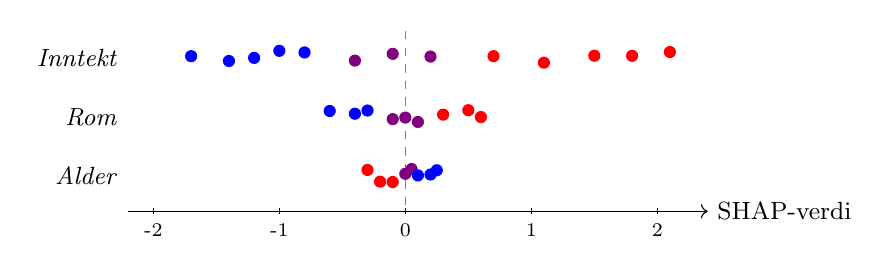
\begin{tikzpicture}[x=1.6cm,y=0.75cm]
\pgfmathsetseed{7}
\draw[->] (-2.2,-0.6) -- (2.4,-0.6) node[right,font=\small] {SHAP-verdi};
\foreach \t in {-2,-1,0,1,2} \draw (\t,-0.55) -- (\t,-0.65) node[below,font=\scriptsize] {\t};
\draw[gray,dashed] (0,-0.5) -- (0,2.5);
\node[left,font=\small] at (-2.2,2) {\emph{Inntekt}};
\node[left,font=\small] at (-2.2,1) {\emph{Rom}};
\node[left,font=\small] at (-2.2,0) {\emph{Alder}};
\foreach \x in {-1.7,-1.4,-1.2,-1.0,-0.8} \fill[blue] (\x,2+0.12*rand) circle (2.2pt);
\foreach \x in {-0.4,-0.1,0.2} \fill[violet] (\x,2+0.12*rand) circle (2.2pt);
\foreach \x in {0.7,1.1,1.5,1.8,2.1} \fill[red] (\x,2+0.12*rand) circle (2.2pt);
\foreach \x in {-0.6,-0.4,-0.3} \fill[blue] (\x,1+0.12*rand) circle (2.2pt);
\foreach \x in {-0.1,0.0,0.1} \fill[violet] (\x,1+0.12*rand) circle (2.2pt);
\foreach \x in {0.3,0.5,0.6} \fill[red] (\x,1+0.12*rand) circle (2.2pt);
\foreach \x in {-0.3,-0.2,-0.1} \fill[red] (\x,0+0.12*rand) circle (2.2pt);
\foreach \x in {0.0,0.05} \fill[violet] (\x,0+0.12*rand) circle (2.2pt);
\foreach \x in {0.1,0.2,0.25} \fill[blue] (\x,0+0.12*rand) circle (2.2pt);
\end{tikzpicture}
\end{center}

Hvilket utsagn er en riktig tolkning av plottet?
\velg{Velg ett alternativ:}
\begin{alternativer}
\alt{A}{\emph{Alder} er viktigst, siden featurene sorteres med den viktigste nederst i et beeswarm-plott}
\alt{B}{Høy \emph{Alder} senker prediksjonen, og \emph{Alder} er den nest viktigste featuren i plottet}
\alt{C}{Høy \emph{Inntekt} øker prediksjonen, og \emph{Inntekt} er den viktigste featuren i plottet}
\alt{D}{Rød farge betyr at SHAP-verdien er positiv, så alle røde punkter i plottet øker prediksjonen}
\end{alternativer}
\sporsmal{3}
Et beslutningstre trenes uten noen begrensning på dybden, og evalueres på de samme dataene:
\begin{lstlisting}[language=Python]
from sklearn.tree import DecisionTreeClassifier
X = [[1, 0], [1, 0], [2, 1], [3, 1], [3, 1], [4, 0]]
y = [0, 1, 1, 0, 0, 1]
tree = DecisionTreeClassifier(random_state=0).fit(X, y)
print(f"{tree.score(X, y):.2f}")
\end{lstlisting}
Hva skrives ut?
\velg{Velg ett alternativ:}
\begin{alternativer}
\alt{A}{\texttt{0.50}}
\alt{B}{\texttt{1.00}}
\alt{C}{\texttt{0.67}}
\alt{D}{\texttt{0.83}}
\end{alternativer}
\sporsmal{4}
Anta at \texttt{X} har shape \texttt{(200, 5)}, \texttt{w} har shape \texttt{(5,)} og \texttt{b} er et tall.

\begin{lstlisting}[language=Python]
z = np.matmul(X, w) + b
y_prob = 1 / (1 + np.exp(-z))
y_pred = [1 if p > 0.3 else 0 for p in y_prob]
\end{lstlisting}

Hvilket utsagn om koden er korrekt?
\velg{Velg ett alternativ:}
\begin{alternativer}
\alt{A}{\texttt{z} har shape \texttt{(200, 5)}, siden hver feature får sin egen score for hvert datapunkt}
\alt{B}{Med terskel 0.3 i stedet for 0.5 kan recall bli lavere, siden færre punkter predikeres positive}
\alt{C}{\texttt{z} har shape \texttt{(200,)}, og verdiene kan være vilkårlige reelle tall, også negative}
\alt{D}{\texttt{y\_pred} inneholder sannsynligheter i intervallet $(0, 1)$ for hvert av de 200 punktene}
\end{alternativer}
\makspoeng

\clearpage
{\sffamily\bfseries\fontsize{18}{22}\selectfont Løsningsforslag}\par\vspace{0.3em}
\noindent\rule{\textwidth}{0.4pt}\par\vspace{1.2em}
Riktig alternativ per spørsmål (bokstaven står i rundingen foran hvert alternativ).\par\vspace{1em}
\begin{center}\sffamily\renewcommand{\arraystretch}{1.35}
\begin{tabular}{l*{4}{>{\centering\arraybackslash}p{1.6cm}}}
\toprule
& \textbf{Sp.\ 1} & \textbf{Sp.\ 2} & \textbf{Sp.\ 3} & \textbf{Sp.\ 4}\\
\midrule
Part 1 & C & D & B & D\\
Part 2 & B & D & B & C\\
Part 3 & D & D & A & C\\
Part 4 & A & B & D & C\\
Part 5 & A & C & A & D\\
Part 6 & B & A & B & B\\
Part 7 & D & C & A & C\\
Part 8 & B & A & C & A\\
Part 9 & B & D & B & A\\
Part 10 & A & C & D & C\\
\bottomrule
\end{tabular}
\end{center}
\end{document}
